\section{Solving Equations}

\begin{frame}[fragile]
\frametitle{Solution of linear equations}
Consider,
  \begin{align*}
    3x + 2y - z  & = 1 \\
    2x - 2y + 4z  & = -2 \\
    -x + \frac{1}{2}y -z & = 0
  \end{align*}
Solution:
  \begin{align*}
    x & = 1 \\
    y & = -2 \\
    z & = -2
  \end{align*}
\end{frame}

\begin{frame}[fragile]
\frametitle{Solving using Matrices}
Let us now look at how to solve this using \texttt{matrices}
  \begin{lstlisting}
In []: A = array([[3,2,-1],
                  [2,-2,4],                   
                  [-1, 0.5, -1]])
In []: b = array([1, -2, 0])
In []: x = solve(A, b)
  \end{lstlisting}
\end{frame}

\begin{frame}[fragile]
\frametitle{Solution:}
\begin{lstlisting}
In []: x
Out[]: array([ 1., -2., -2.])
\end{lstlisting}
\end{frame}

\begin{frame}[fragile]
\frametitle{Let's check!}
\begin{small}
\begin{lstlisting}
In []: Ax = dot(A, x)
In []: Ax
Out[]: array([ 1.00000000e+00,  -2.00000000e+00, 
              -1.11022302e-16])
\end{lstlisting}
\end{small}
\begin{block}{}
The last term in the matrix is actually \alert{0}!\\
We can use \texttt{allclose()} to check.
\end{block}
\begin{lstlisting}
In []: allclose(Ax, b)
Out[]: True
\end{lstlisting}
\end{frame}

\begin{frame}[fragile]
\frametitle{\texttt{roots} of polynomials}
\begin{itemize}
\item \texttt{roots} function can find roots of polynomials
\item To calculate the roots of $x^2-5x+6$ 
\end{itemize}
\begin{lstlisting}
  In []: coeffs = [1, -5, 6]
  In []: roots(coeffs)
  Out[]: array([3., 2.])
\end{lstlisting}
\vspace*{-.2in}
\begin{center}
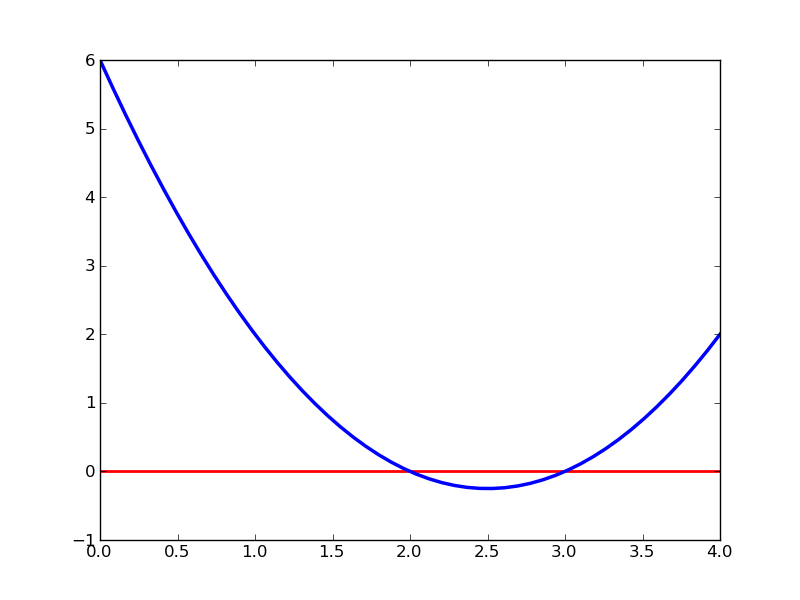
\includegraphics[height=1.6in, interpolate=true]{images/roots}    
\end{center}
\end{frame}

\begin{frame}[fragile]
\frametitle{SciPy: \texttt{fsolve}}
\begin{small}
\begin{lstlisting}
  In []: from scipy.optimize import fsolve
\end{lstlisting}
\end{small}
\begin{itemize}
\item Finds the roots of a system of non-linear equations
\item Input arguments - Function and initial estimate
\item Returns the solution
\end{itemize}
\end{frame}

\begin{frame}[fragile]
\frametitle{\texttt{fsolve} \ldots}
Find the root of $sin(z)+cos^2(z)$ nearest to $0$
\begin{lstlisting}
In []: def g(z):
 ....:     return sin(z)+cos(z)*cos(z)

In []: fsolve(g, 0)
Out[]: -0.66623943249251527
\end{lstlisting}
\begin{center}
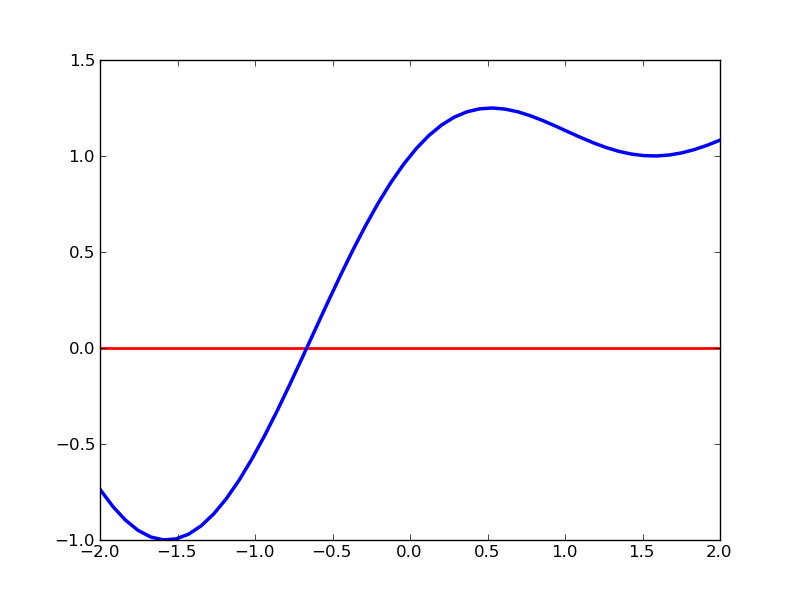
\includegraphics[height=2in, interpolate=true]{images/fsolve}    
\end{center}
\end{frame}

\section{ODEs}

\begin{frame}[fragile]
\frametitle{Solving ODEs using SciPy}
\begin{itemize}
\item Consider the spread of an epidemic in a population
\item $\frac{dy}{dt} = ky(L-y)$ gives the spread of the disease
\item $L$ is the total population.
\item Use $L = 2.5E5, k = 3E-5, y(0) = 250$
\item Define a function as below
\end{itemize}
\begin{lstlisting}
In []: from scipy.integrate import odeint
In []: def epid(y, t):
  ....     k = 3.0e-5
  ....     L = 2.5e5
  ....     return k*y*(L-y)
  ....
\end{lstlisting}
\end{frame}

\begin{frame}[fragile]
\frametitle{Solving ODEs using SciPy \ldots}
\begin{lstlisting}
In []: t = linspace(0, 12, 61)

In []: y = odeint(epid, 250, t)

In []: plot(t, y)
\end{lstlisting}
%Insert Plot
\end{frame}

\begin{frame}[fragile]
\frametitle{Result}
\begin{center}
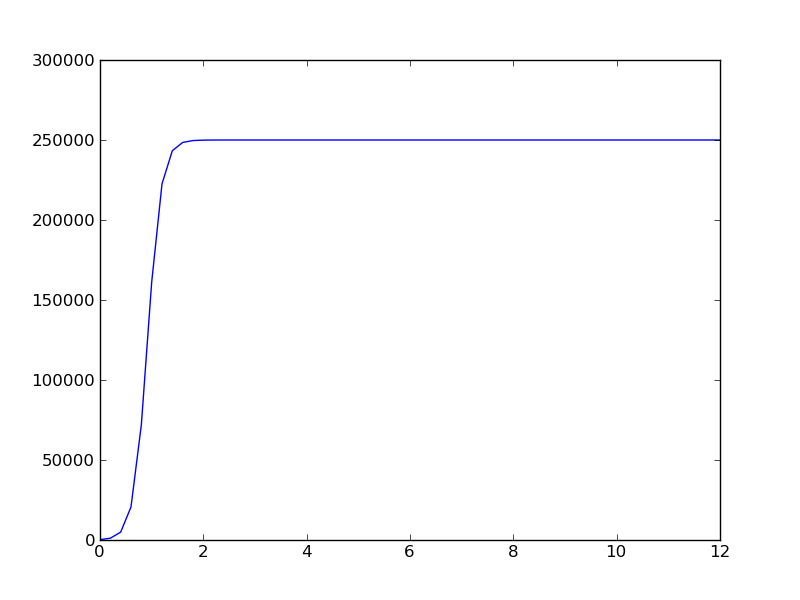
\includegraphics[height=2in, interpolate=true]{images/epid}  
\end{center}
\end{frame}


\begin{frame}[fragile]
\frametitle{ODEs - Simple Pendulum}
We shall use the simple ODE of a simple pendulum. 
\begin{equation*}
\ddot{\theta} = -\frac{g}{L}sin(\theta)
\end{equation*}
\begin{itemize}
\item This equation can be written as a system of two first order ODEs
\end{itemize}
\begin{align}
\dot{\theta} &= \omega \\
\dot{\omega} &= -\frac{g}{L}sin(\theta) \\
 \text{At}\ t &= 0 : \nonumber \\
 \theta = \theta_0(10^o)\quad & \&\quad  \omega = 0\ (Initial\ values)\nonumber 
\end{align}
\end{frame}

\begin{frame}[fragile]
\frametitle{ODEs - Simple Pendulum \ldots}
\begin{itemize}
\item Use \texttt{odeint} to do the integration
\end{itemize}
\begin{lstlisting}
In []: def pend_int(initial, t):
  ....     theta = initial[0]
  ....     omega = initial[1]
  ....     g = 9.81
  ....     L = 0.2
  ....     F=[omega, -(g/L)*sin(theta)]
  ....     return F
  ....
\end{lstlisting}
\end{frame}

\begin{frame}[fragile]
\frametitle{ODEs - Simple Pendulum \ldots}
\begin{itemize}
\item \texttt{t} is the time variable \\ 
\item \texttt{initial} has the initial values
\end{itemize}
\begin{lstlisting}
In []: t = linspace(0, 20, 101)
In []: initial = [10*2*pi/360, 0]
\end{lstlisting} 
\end{frame}

\begin{frame}[fragile]
\frametitle{ODEs - Simple Pendulum \ldots}
%%\begin{small}
\texttt{}
%%\end{small}
\begin{lstlisting}
In []: from scipy.integrate import odeint
In []: pend_sol = odeint(pend_int, 
                         initial,t)
\end{lstlisting}
\end{frame}

\begin{frame}[fragile]
\frametitle{Result}
\begin{center}
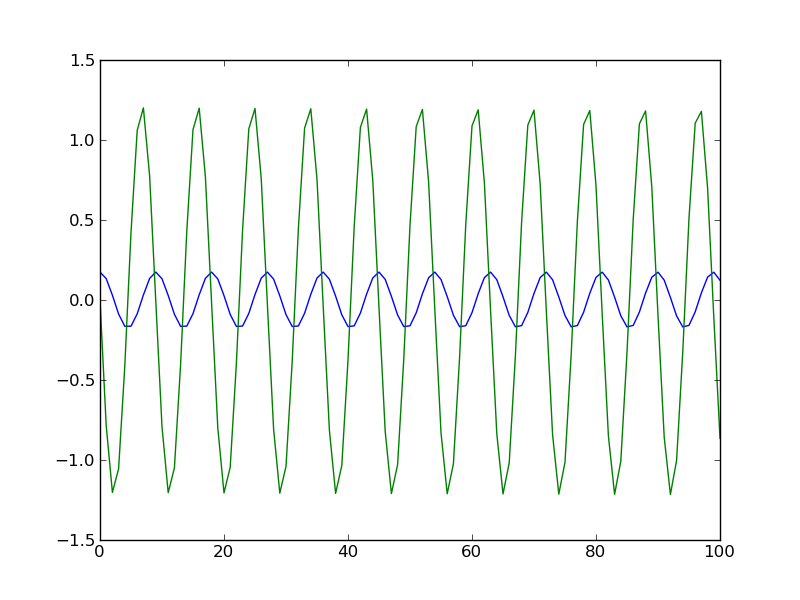
\includegraphics[height=2in, interpolate=true]{images/ode}  
\end{center}
\end{frame}

%% \section{FFTs}

%% \begin{frame}[fragile]
%% \frametitle{The FFT}
%% \begin{itemize}
%%     \item We have a simple signal $y(t)$
%%     \item Find the FFT and plot it
%% \end{itemize}
%% \begin{lstlisting}
%% In []: t = linspace(0, 2*pi, 500)
%% In []: y = sin(4*pi*t)

%% In []: f = fft(y)
%% In []: freq = fftfreq(500, t[1] - t[0])

%% In []: plot(freq[:250], abs(f)[:250])
%% In []: grid()
%% \end{lstlisting} 
%% \end{frame}

%% \begin{frame}[fragile]
%% \frametitle{FFTs cont\dots}
%% \begin{lstlisting}
%% In []: y1 = ifft(f) # inverse FFT
%% In []: allclose(y, y1)
%% Out[]: True
%% \end{lstlisting} 
%% \end{frame}

%% \begin{frame}[fragile]
%% \frametitle{FFTs cont\dots}
%% Let us add some noise to the signal
%% \begin{lstlisting}
%% In []: yr = y + random(size=500)*0.2
%% In []: yn = y + normal(size=500)*0.2

%% In []: plot(t, yr)
%% In []: figure()
%% In []: plot(freq[:250],
%%   ...:      abs(fft(yn))[:250])
%% \end{lstlisting}
%% \begin{itemize}
%%     \item \texttt{random}: produces uniform deviates in $[0, 1)$
%%     \item \texttt{normal}: draws random samples from a Gaussian
%%         distribution
%%     \item Useful to create a random matrix of any shape
%% \end{itemize}
%% \end{frame}

%% \begin{frame}[fragile]
%% \frametitle{FFTs cont\dots}
%% Filter the noisy signal:
%% \begin{lstlisting}
%% In []: from scipy import signal
%% In []: yc = signal.wiener(yn, 5)
%% In []: clf()
%% In []: plot(t, yc)
%% In []: figure()
%% In []: plot(freq[:250], 
%%   ...:      abs(fft(yc))[:250])
%% \end{lstlisting}
%% Only scratched the surface here \dots
%% \end{frame}
